\documentclass{article}

\usepackage{geometry}
\geometry{margin=2cm}
\usepackage{graphicx}
\usepackage{hyperref}
\usepackage{amsfonts}
\usepackage{caption}
\usepackage{subcaption}

\hypersetup{colorlinks=true, linkcolor=blue, urlcolor=blue}
\urlstyle{same}
\begin{document}
	
	\author{Aayush Arya}
	\date{(Submitted: \today)}
	\title{}
	
	\maketitle
	
	\hrule
	\begin{center}
		PHY366 Lab Report\\
		Practical: 9 \quad Registration No.: 11912610 \quad Section: G2903
	\end{center}
	\hrule
	
	\section*{Aim}
	To profile the output and transfer characteristics of a JFET.
	
	\section*{Methods}
	
	A JFET circuit with an n-channel was constructed. The circuit is available at \url{https://www.multisim.com/content/RyER9NMjAwDDNWqQmnkheN/output-charactersitics-of-jfet/open/} and is shown in Figure \ref{fig:circuit}.
	
	\begin{figure}[!h]
		\centering
		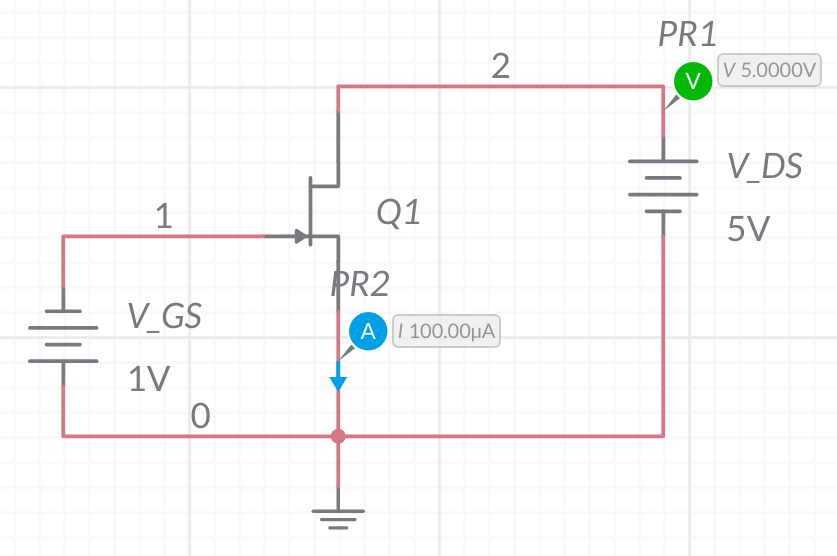
\includegraphics[width=0.7\textwidth]{jfet_circuit}
		\caption{Circuit diagram of the n-channel JFET}
		\label{fig:circuit}
	\end{figure}
	
	For the output characterisation, we studied the JFET in the shorted input ($V_{GS} =0$) configuration and then also varied $V_{GS}$ to obtain characteristics for different input voltages.
	
	\section*{Results \& Conclusions}
	
	We show the output and transfer characteristics in Figure \ref{fig:out}. It is evident that in the short-circuit configuration (i.e. $V_{GS} = 0$) the drain current saturates at $I_{DSS} = 400\mu$A. The corresponding pinch voltage occurs at $V_{DS} = 2$V, which we highlight using a grey dotted vertical line.\\
	
	Clearly, if the input is set to the pinch voltage (i.e., 2V), the output current vanishes, which is consistent with what we expect from the relation\[ I_D = I_{DSS}\left( 1 - \frac{V_{GS}}{V_p} \right)^2 \]
	
	from the expression we also see that $I_D$ is not a linear function of the input $V_{GS}$, a phenomenon that is evident in the transfer characteristics (also shown in Figure \ref{fig:out}).
	
	\begin{figure}[h!]
		\centering
		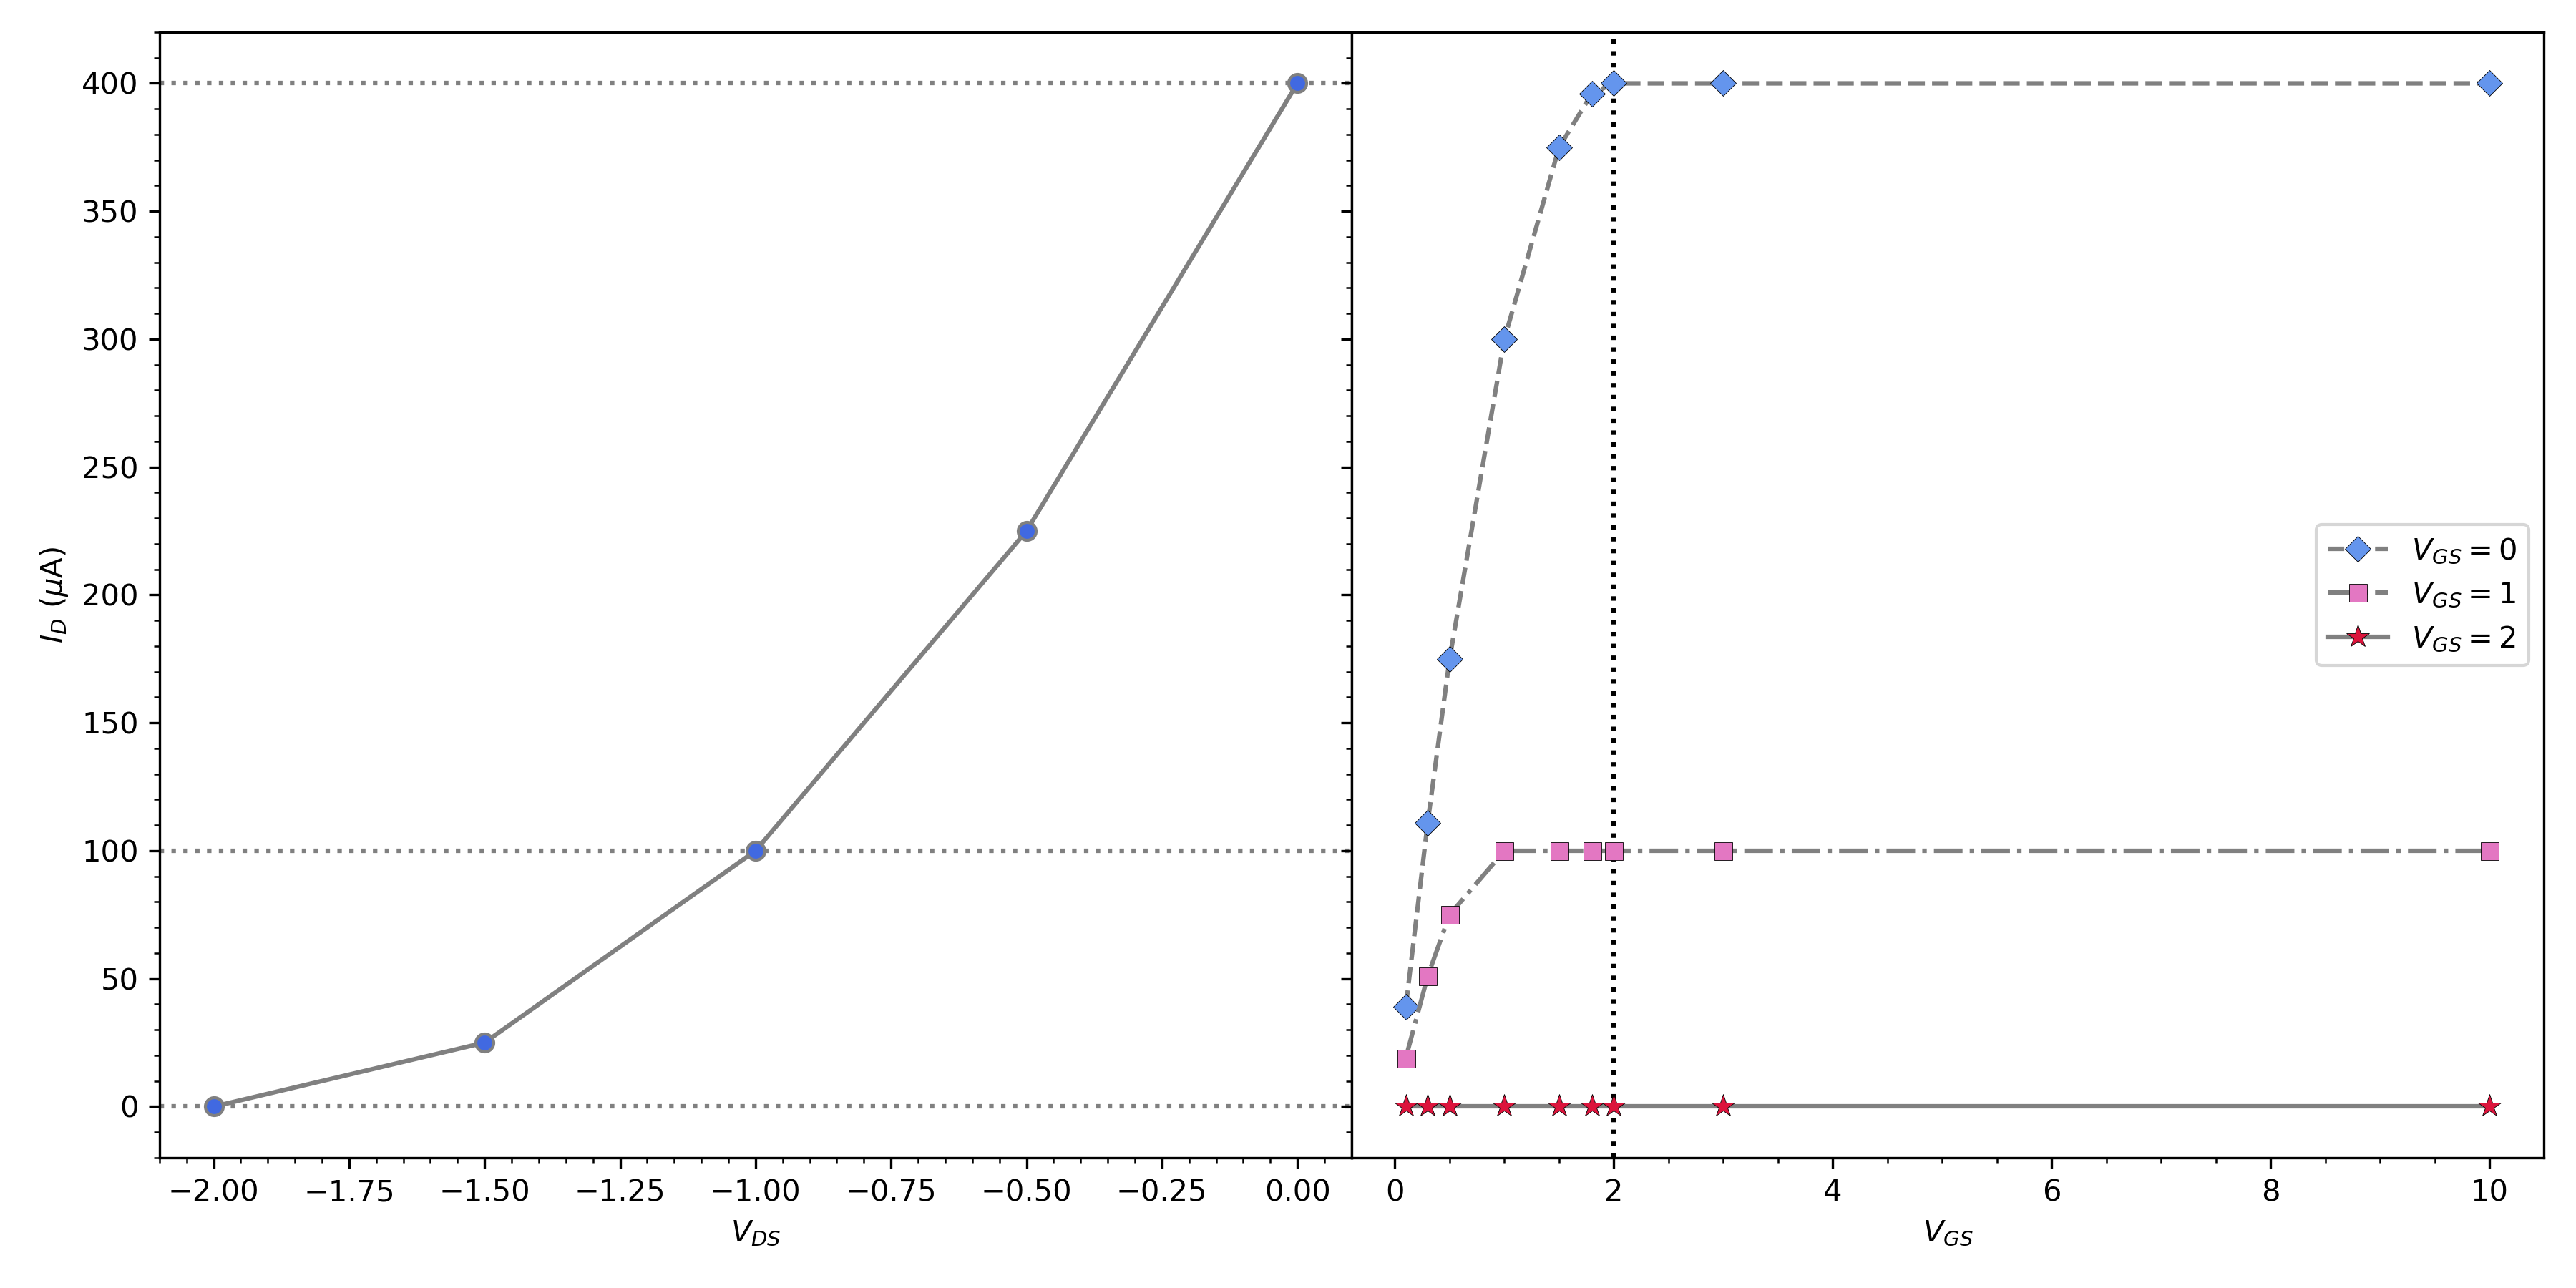
\includegraphics[width=0.9\textwidth]{output_chars}
		\caption{The transfer (left) and output (right) characteristics of the JFET. The pinch voltage $V_p$ for the short-circuit configuration was clearly found to be $V_p = 2$V. The dotted vertical line shows the pinch voltage for the shorted input configuration.}
		\label{fig:out}
	\end{figure}

	
	The transfer characteristics show a non-linear relationship of $I_D$ with $V_{GS}$. These were obtained by finding the saturation points of $I_D$ for different input $V_{GS}$.
	
	
	\begin{table}[!h]
		\centering
		\begin{tabular}{|c|c|c|c|}
		\hline
			$V_{DS}$ (V) & \multicolumn{3}{c}{$I_D$ ($\mu$A)} \\
			\hline
			& $V_{GS}=0$     & $V_{GS}=1$     & $V_{GS}=2$     \\
		\hline
			0.10         & 39          & 19          & $-2.01\times 10^{-6}$      \\
			0.30         & 111         & 51          & ..             \\
			0.50         & 175         & 75          & ..             \\
			1.00         & 300         & 100         & ..             \\
			1.50         & 375         & 100         & ..             \\
			1.80         & 396         & 100         & ..             \\
			2.00         & 400         & 100         & ..             \\
			3.00         & 400         & 100         & ..             \\
			10.00        & 400         & 100         & $-2.01\times 10^{-6}$\\
		\hline
		\end{tabular}
		\caption{The output characteristics measurements.}
		\label{tab:out}
	\end{table}
	
	The measurements for the output characteristics have been summarized in Table \ref{tab:out}.
	
\end{document}